On souhaite déterminer le point de contact $R$ d'un rayon partant d'une source $S$ et passant par un point d'incidence $I$ après réflexion sur un miroir sphérique $\setgeo{S}$ de centre $\Omega$. Il est évident que l'on peut raisonner dans le plan formé par les points $\Omega$, $S$ et $I$, et considérer le cercle $\setgeo{C}$ intersection de $\setgeo{S}$ avec ce plan.

\medskip

\begin{center}
	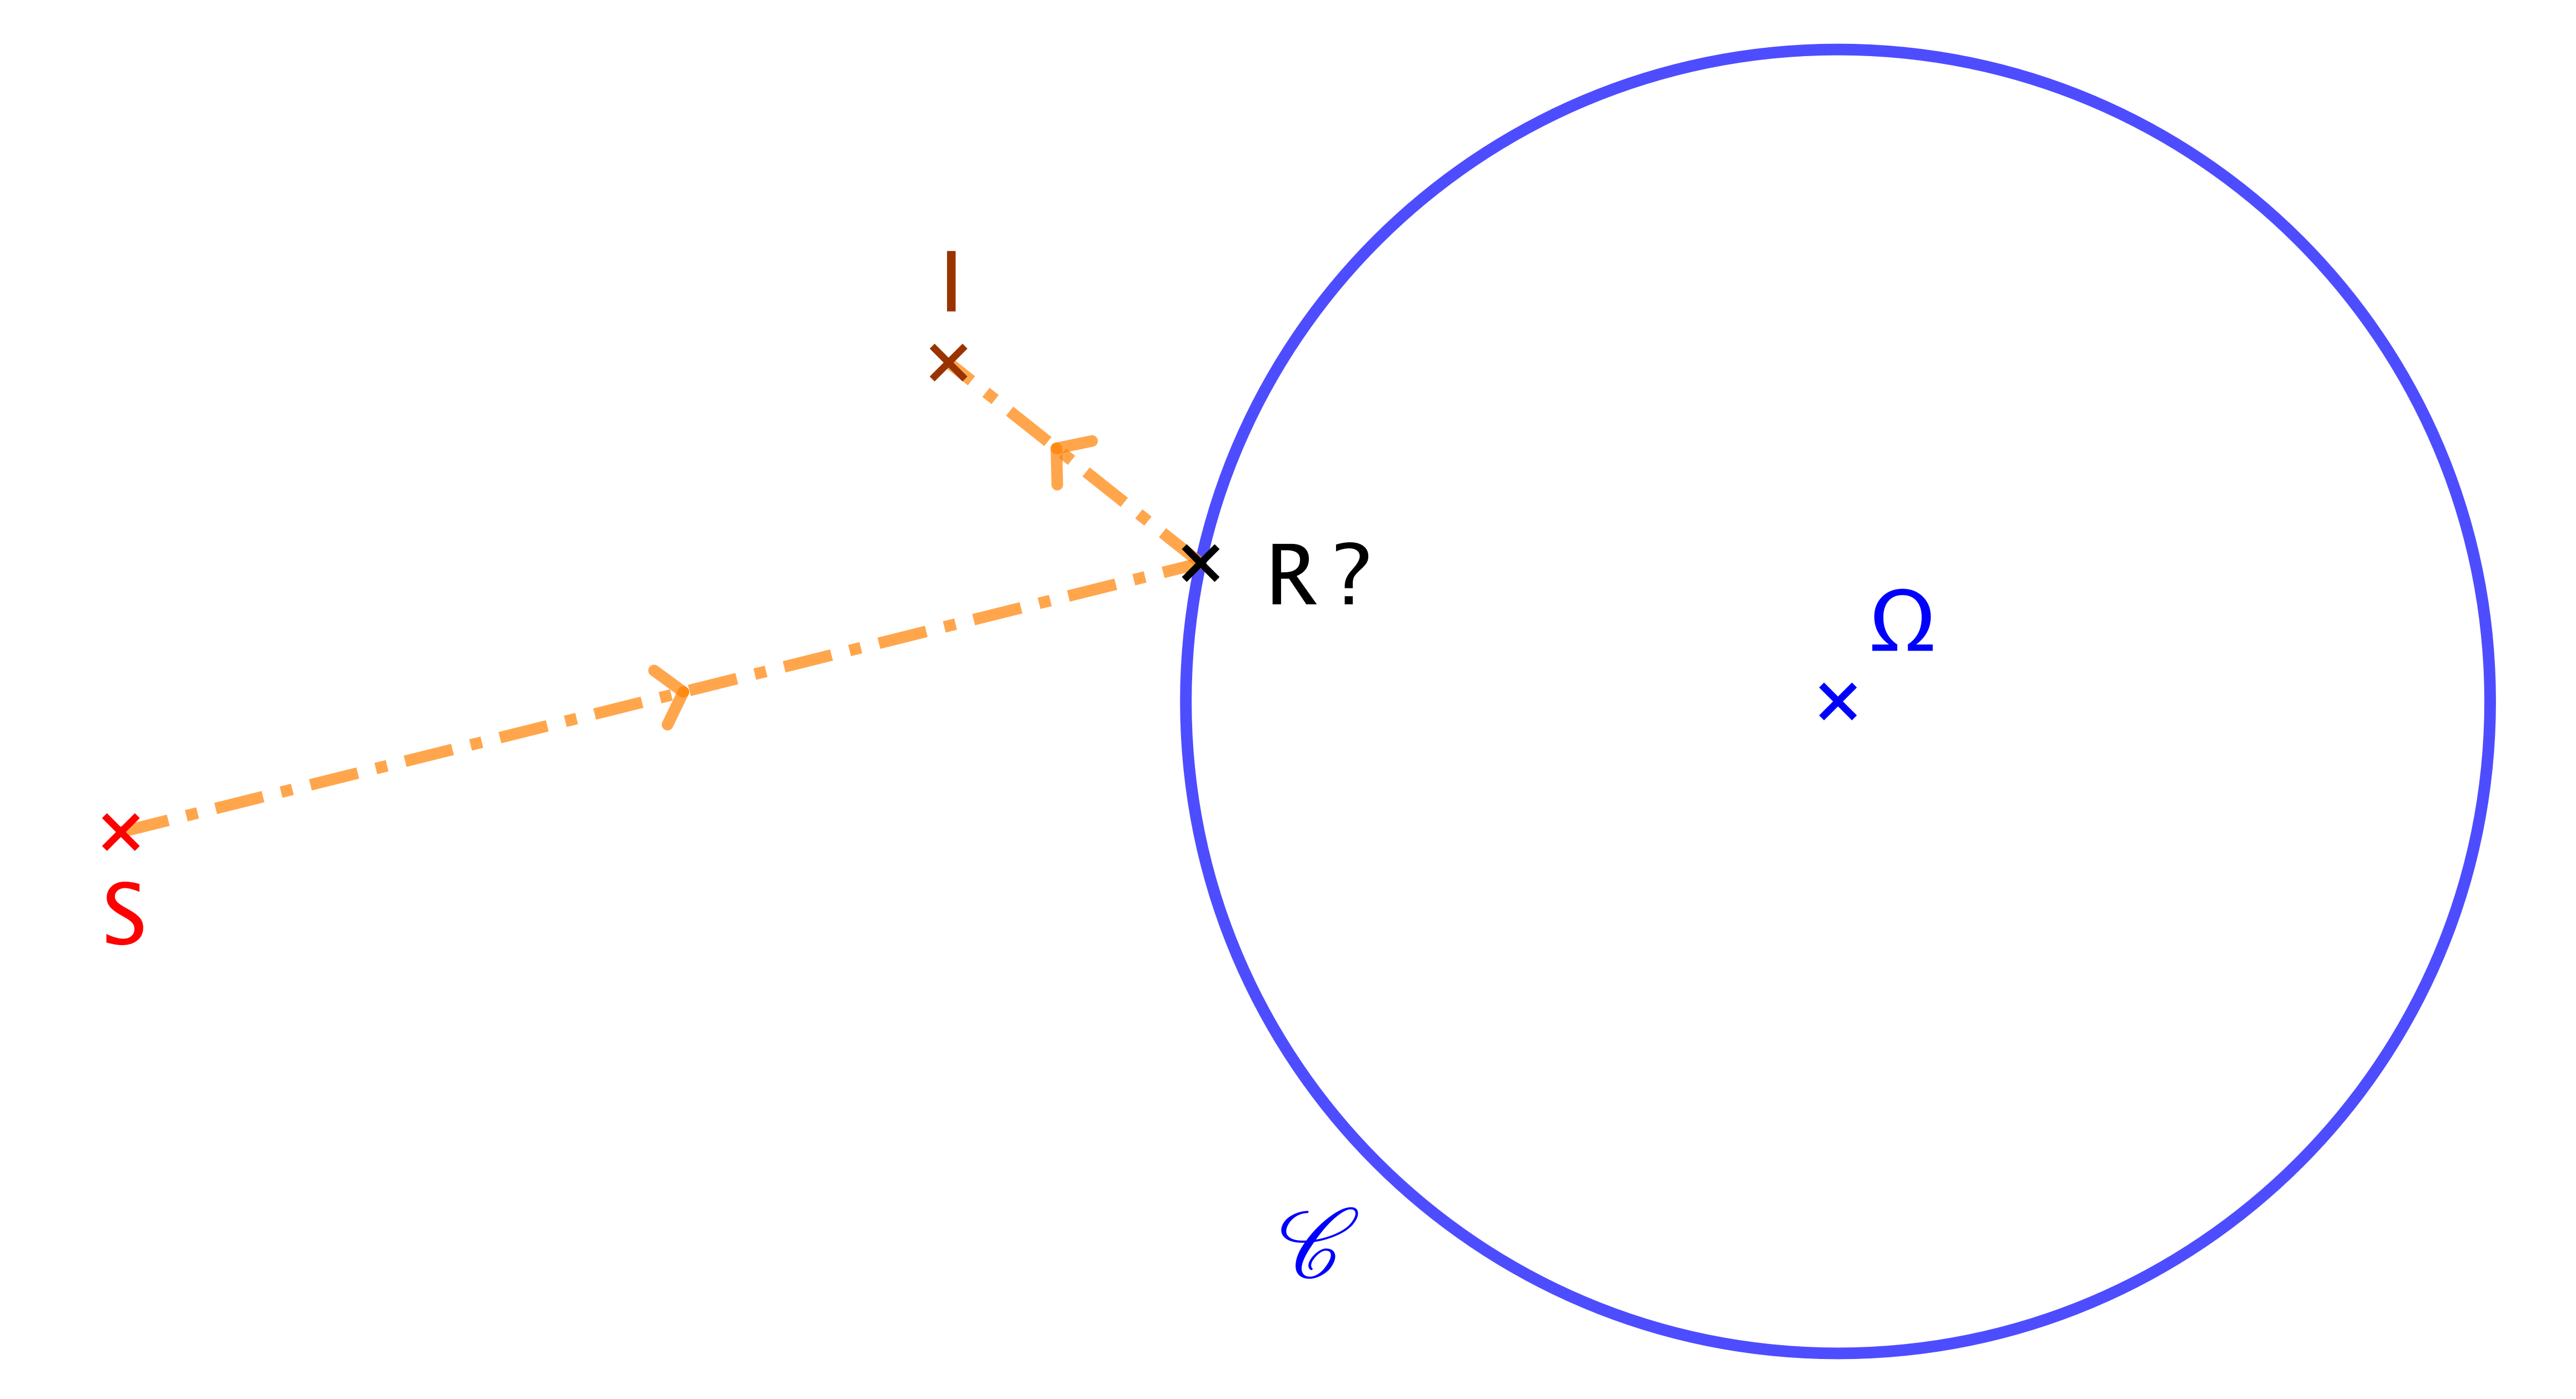
\includegraphics[scale=.75]{intro.png}
\end{center}
